\chapter{Introduction}

This bachelor thesis deals with an implementation of Netbeans plugin which will be used for class modeling. I chose this theme because of two main reasons. The first reason is that it is not a standard information system (or something similar) that can be created with no need to learn new technologies (these systems are based on usage of well-known common frameworks). In this project I will learn to work with new frameworks like JGraph (section \ref{section:JGraph}) and Netbeans Platform (section \ref{section:netbeansAPI}). The second reason is that this project can produce an useful system which can be extended e.g. within the scope of another thesis. Of course, the result of one bachelor thesis cannot produce more sophisticated system than the existing (paid) ones, but it provides a good basis for further expansion. 

At the beginning I would like to point out that this work is not a recherche one. I didn't try to compare several possible solutions of the problem but I tried to create a solution of the problem. Despite the fact that I have been inspired by several existing systems, these systems are not described in a detail. In this thesis I focused on the description of the implementation and thus it should be easy to implement similar system according to it.

The structure of this thesis is divided into two main parts. The first part is called Analysis. This part contains the information about the functionality of the program from the view of the user, a little info about existing solutions that inspired me, used frameworks and some of used design patterns.

The second part is called Application and consists of implementation documentation. In this part there is a description of how the system works inside and of some interesting subsystems.

\section{Class Diagram}
\label{section:classDiagramDescription}

A class diagram is a basic UML\footnote{UML - Unified Modeling Language} diagram. It is probably the best known of all UML diagrams. The class diagram is used for description of system's (or program's) structure by showing its classes and their relations. In a computer engineering, class diagram is used for both conceptual modeling (business modeling) and class modeling on platform level, which is consequently translated into a programming language (into the programming code).

Conceptual modeling is frequently used in early stage of software/system development. Its purpose is to depict the basic ideas of the domain that we want to build (a problem domain). It is why is this model often called Domain Object Model (DOM) or simply domain model. The domain model represents the vocabulary and key features of the problem domain. These features are represented by entities that occur in the problem domain, their attributes and relations between them. This type of model is really useful as a communication tool between several members of business team or between the business and technical team. By this model it can be also verified that the system meets the user's requirements, but only if this model is created well.

Despite the fact that the diagram is called class diagram, it does not describe only the classes of the system. It describes all the data types like interfaces, enumeration types, etc. Concrete types (class, interface, etc.) are distinguished by stereotypes. All these data types are in the class diagram displayed as rectangles. These rectangles can be divided into three parts: 
\begin{itemize}
    \item The first part contains the name of the class (or interface, enumeration, etc.) and eventually the stereotype (a text in \guillemotleft angle quotes\guillemotright) which describes a special property (interface, enumeration, or something else). If there is no stereotype, it means that the rectangle represents a simple class.
    \item The second part contains the list of attributes. Every attribute defines its scope (public, private, protected), name and the data type. There don't have to be all the attributes in this part, but only the important ones.
    \item The last, third part, contains the list of methods. Every method defines its scope, name, list of parameters and the return value. Again, there can be only methods which are important to depict a concrete problem.
\end{itemize}

\begin{figure}[!ht]
\begin{center}
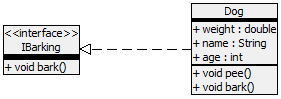
\includegraphics[]{img/classDiagramExample.png}
\caption{Example of a class diagram}
\label{f-classDiagramExample}
\end{center}
\end{figure}

Example of a class diagram (on Java platform level) can be seen in the Figure \ref{f-classDiagramExample}. There are two rectangles. First, with name IBarking, represents the interface (it has the \guillemotleft{}interface\guillemotright stereotype). This interface defines one public method with no return type (void) called bark. The second rectangle represents simple class (there is no stereotype) called Dog. The Dog class defines three public attributes (weight of the double type, name of the String type and age of the integer type) and two public methods (pee and bark), both with no return type. Between these two rectangles there is a relationship defining that the Dog class implements the IBarking interface. More information about class diagram can be found in \cite{UMLDistilled}.
